\section{Elaboration}
%--------------------------------------------------------------------------------







\subsection{Basics}
%--------------------------------------------------------------------------------

After parsing we get an abstract syntax tree (AST) of the source file. Each
subterm of the AST gets a source based metavariable, a goal and a task which
elaborates the source term. Source based metavariables are never instantiated by
constraint solving. Source based metavariable are instantiated at the end of the
corresponding task.

The elaborator can create more metavariables for the following reasons:

\begin{enumerate}
    \item Missing type information in the source code.

    \item Implicit function arguments not explicitly provided in the source code.

    \item Wild cards in the source code (the wild card {\tt \_} is a request
        from the programmer to the compiler to fill in the information).

    \item Intermediate metavariables introduced during unification for subterms
        in an imitation step where the pattern on flex side include variables
        regarded as constants.

    \item Pattern variables in case trees.
\end{enumerate}

The instantiation of metavariables is used to synchronize the tasks in the
elaborator. A task can be blocked because it is waiting for one or more
metavariables to be instantiated (e.g. when the metavariable is the head term
and head normal form is required). A task which instantiates a metavariable
unblocks all tasks which wait for the instantiation of the metavariable.

Finally either all metavariables are instantiated or a deadlock is reached
because the wait-for graph has become cyclic.

The wait-for graph for source based metavariables can never become cyclic
because source based metavariables have a clear hierarchy given by the AST.
Therefore if the programmer provides all type information and all implicit
arguments explicitly a dead lock can never
appear. A deadlock appears if the compiler cannot elaborate the missing
information.

Metavariables representing missing information must have enough source code
information to generate a useful error message. If a deadlock occurs, the
elaborator searches for the first metavariable representing missing
information and prints an error message.






\subsection{Definitions}
%--------------------------------------------------------------------------------


A definition has the form
$$
    \Gamma \vdash f \vec {x^A}. R := e
$$

There are local and global definitions. For a local definition we have to find a
definition term of the form $\lambda \vec {x^A}. e: \Pi \vec{x^A}. R$ which
contains only metavariables defined in the context $\Gamma$ in order to be
entered into the context $\Gamma$ and to proceed with the rest of the term.
A local definition is part of a let expression
$$
    \letbr{z^C := c, b}
$$
and we need the definition term $c$ and its type $C$ to elaborate the body $b$.

For a local definition we want the definition of the form (details see below)
$$
    f
    :
    \Pi \vec {w^C}. M_R \vec w
    :=
    \lambda \vec{w^C}. m_{\hat e} \vec w
$$
where all metavariables are valid in the outer context $\Gamma$.

For a global definition the definition is needed in the form
$$
    f: \Pi \vec{x^A} . R := \lambda \vec {x^A}. e
$$
which does not contain any metavariables.



The elaboration has the following steps:

\begin{enumerate}

    \item Elaborate the formal arguments:

        We elaborate the formal arguments left to right and use the following
        abbreviations
        $$
            \vertlist{
                \vec a &=&
                [x_i^{A_i}, \ldots]
                \\
                \vec {v^B} &=& [x_0^{B_0}, \ldots, x_{i-1}^{B_{i-1}}]
                \\
                \vec {v^C} &=& [x_0^{C_0}, \ldots, x_{i-1}^{C_{i-1}}]
            }
        $$
        where $\vec a$ is the list of not yet elaborated formal arguments,
        $\vec { v^B}$ is the list of elaborated formal arguments which contain
        local metavariables and $\vec {w^C}$ is the optional list of formal
        arguments which do not contain local metavariables (they contain only
        metavariables valid in the outer context $\Gamma$. For local defintions
        the list $\vec {w^C}$ is needed.

        The elaboration starts with
        $$
            \vertlist{
                \vec a &=& \vec {x^A}
                \\
                \vec {v^B} &=&  []
                \\
                \vec {v^C} &=&  []
            }
        $$

        Now we iterate over all formal arguments. On each step where the list of
        not yet elaborated formal arguments is
        $$
            x^A \vec a
        $$
        we do the following steps:

        \begin{enumerate}
            \item We create the metavariable $N_A$ with
                $$
                \Gamma, \vec {v^B} \vdash N_A : \Box_0
                $$
                and spawn a task to elaborate $A$ into $N_A$ in case $A$ is
                present in the source code.

            \item Optionally we create the metavariable $M_A$ with
                $$
                    \Gamma \vdash M_A: \Pi \vec {w^C}. \Box_0
                $$
                and spawn a task to unify $N_A$ with $M_A \vec{v}$ in the inner
                context $\Gamma, \vec{v^B}$.

            \item Return $\vec {v^B} x^{N_A}$ and optionally
                $\vec {w^C} x^{M_A \vec w}$.

        \end{enumerate}

        After processing all formal arguments we get $\vec{v^B}$ and optionally
        $\vec {w^C}$.



    \item Elaborate the result type:

        \begin{enumerate}

            \item Create the metavariable $N_R$ with
                $$
                    \Gamma, \vec{v^B} \vdash N_R : \Box_0
                $$
                and spawn a task to elaborate the result type $R$ into $N_R$ in
                case $R$ is present in the source code.

            \item Optionally create the metavariable $M_R$ with
                $$
                    \Gamma \vdash M_R : \Pi \vec{v^C}. \Box_0
                $$
                and spawn a task to unify $N_R$ with $M_R \vec v$ in the inner
                context.
        \end{enumerate}



    \item Elaborate the body:

        We have reached the state where we have the formal arguments and a
        metavariable representing the result type
        $$
            \vertlist{
                \vec {v^B}
                \\
                \vec {w^C} & &
                & \text {local def}
                \\
                \Gamma, \vec {v^B} &\vdash & N_R : \Box_0
                \\
                \Gamma &\vdash& M_R : \Pi \vec{w^C}. \Box_0
                &\text{local def}
            }
        $$

        \begin{enumerate}
            \item Define the metavariable $m_e$ with
                $$
                    \Gamma, \vec{v^B}, f^{N_R}
                    \vdash
                    m_e : N_R
                $$
                and spawn a task to elaborate the body $e$ into $m_e$.

            \item Optionally define the metavariable $m_{\hat e}$ with
                $$
                    \Gamma \vdash m_{\hat e}: \Pi \vec {w^C}. M_R \vec x
                $$

            \item Spawn a task which:
                \begin{itemize}
                    \item waits for $m_e$.

                    \item checks if $f$ is only legally used in the body (i.e.
                        only calls with structurally smaller arguments).

                    \item if $f$ is used in the body then it returns
                        $$
                            \fixbr{f^{N_R}, m_e}
                        $$
                        otherwise it returns $m_e$.

                    \item optionally waits for all local
                        metavariables in the result to be filled and then fills
                        $m_{\hat e}$ with
                        $$
                            \lambda \vec {w^C}. r
                        $$
                        where $r$ is the result.
                \end{itemize}
        \end{enumerate}


    \item Enter a local definition:


    \item Enter a global definition:


\end{enumerate}








\subsection{Abstractions}
%--------------------------------------------------------------------------------

$$
\Gamma \vdash \lambda x^A. e^E : R
$$

The type annotations $A$ and $E$ are optional.

An elaboration can be successful only if it elaborates a term which satifies the
requirement $R$. There are only two possibilities to satisfy the requirement.

\begin{enumerate}
    \item $R$ represents a function type i.e. it has the form $\Pi x^{A_r}.
        B_r$. In that case the requirement can flow down to give requirements
        for $A$, $E$ and $e$.

    \item $R$ has a metavariable $\meta M$ as a head term and $R$ is a pattern
        i.e. $R = \meta M \vec y$ where $\vec y$ are pairwise distinct free
        variables. In that case the requirement can flow up. I.e. the
        elaboration elaborates a term with the type $\Pi x^A. B$ and the
        unification of the type with $R$ instantiates $\meta M$.
\end{enumerate}


\begin{enumerate}
    \item $R = \Pi x^{A_r}. B_r$: I.e. the required type is a function type.

        \begin{enumerate}
            \item If $A$ is present then elaborate $A$ with $\Gamma \vdash A_r
                \le A$. Otherwise use $A = A_r$.

            \item If $E$ is present then elaborate $E$
                with $\Gamma, x^A \vdash E \le B_r$. Otherwise use $E = B_r$.

            \item Elaborate $e$ with $\Gamma, x^A \vdash e: E$.

            \item Form $\Gamma \vdash \lambda x^A. e^E : \Pi x^A. E$ where $\Pi
                x^A. E$ is guaranteed to be a subtype of $\Pi x^{A_r}. B_r$.

                The forming of $\lambda x^A. e^E$ requires that all
                metavariables belonging to the context $\Gamma, x^A$ are
                instantiated. This usually requires waiting (e.g. $e$ is usually
                an application where the metavariables representing arguments
                have to be instantiated).
        \end{enumerate}

    \item $R = \meta M \vec a$: The required type is represented by an
        uninstantiated metavariable $\meta M$.

    \item All other cases are error cases.

        Open question: What happens with a stuck case tree application?
\end{enumerate}





\subsection{Applications}
%---------------------------------------------------------------------------

$$ f a$$


The elaborator of $f a$ starts with a signature requirement $[R]$ and
an optional required type.

\paragraph{Subtasks}
\begin{enumerate}
    \item $E_f$: Elaborate $f$
    \item $E_a$: Elaborate $a$
    \item $U_{A}$: Unify the type of $a$ as a subtype of the argument type of
        $f$
    \item $U_{R}$: Unify the type of $\meta f \meta a$ as a subtype of the
        required type of $fa$.
    \item $E_{fa}$: Elaborate $fa$
\end{enumerate}

The subtasks $E_f$, $U_A$, $U_R$ and $E_{fa}$ have to be executed in sequence. The
subtask $E_a$ can run interleaved.


\paragraph{Algorithm}
\begin{enumerate}
    \item Make holes:
        \begin{enumerate}
            \item Make the unkown signature element $\meta U$.

            \item Make a hole $\meta f$ for $f$ with signature requirement $[\meta U, R]$.

            \item Make a hole $\meta A$ for the type of $a$ with the signature
                requirement $[S]$.

            \item Make a hole $\meta a$ for $a$ with signature requirement $[\meta U]$
                and the
                required type $\meta A$.
        \end{enumerate}

    \item Waiting tasks:
        \begin{enumerate}
            \item Put $U_{A}$ into the wait queue for $\meta f$.

            \item Put $U_R$ into the wait queue for $U_A$.

            \item Put $E_{fa}$ into the wait queue for $U_R$.
        \end{enumerate}

    \item Ready tasks:
        \begin{enumerate}
            \item Push $E_a$ into the ready queue.

            \item Push $E_f$ into the ready queue.
        \end{enumerate}
\end{enumerate}


\paragraph{Remarks}

\begin{itemize}
    \item The elaborators of $f$ and $a$ don't have any preconditions. For the
        result of the elaboration the sequence is not important. However it is
        preferable to start the elaboration of $f$ before the elaboration of
        $a$. The elaboration of $a$ has a better chance to be successful without
        becoming stuck if the elaboration of $f$ has finished and the required
        type $\meta A$ for $a$ is available.

    \item The term $fa$ can be built as soon as the type of $a$ is unified with
        the argument type of $f$ and the type of $\meta f \meta a$ is unified
        with the required result type. Before that it is not evident that $fa$ is
        welltyped and satisfies its requirement.
\end{itemize}




\paragraph{Example}
%------------------------------------------------------------
Elaborate the term
\begin{alba}
    (|>) 1 (+) 2: Nat

    -- equivalent to
    (1 |> (+)) 2: Nat

    -- in global context
    (+): Nat -> Nat -> Nat
    (+): String -> String -> String)

    (|>) {A: Any} {P: A -> Any} (a: A) (f: all x: P x): P a
    :=
        f a
\end{alba}

\resizebox{8cm}{3cm}{
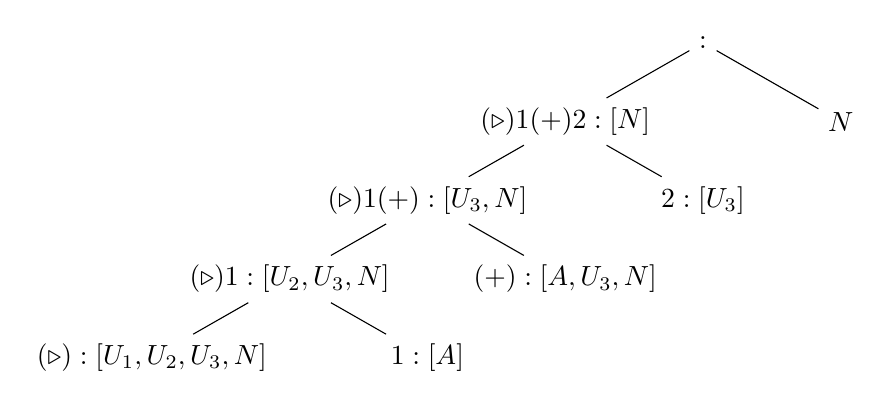
\begin{tikzpicture}
    \def\app{{\scriptsize app}}
    \def\f{{(\triangleright)}}
    \def\p{{(+)}}
    \node {:} [sibling distance = 3.5cm, level distance = 1cm]
        child {node {$\f 1 \p 2:[N]$}
            child {node {$\f 1 \p:[U_3, N]$}
                child {node {$\f 1:[U_2, U_3, N]$}
                    child {node {$\f: [U_1,U_2,U_3,N]$}}
                    child {node {$1: [A]$}}
                }
                child {node {$(+): [A,U_3,N]$}}
            }
            child {node {$2: [U_3]$}}
        }
        child {node {$N$}};
\end{tikzpicture}
}

We start with the elaboration of $(\triangleright) 1 (+) 2$ with the signature
requirement $[N]$ and the required type $N$.

\begin{itemize}
    \item The term is an application with the function term $(\triangleright) 1
        (+)$ and the argument $2$. We start the elaboration of the function term
        with the signature requirement $[U_3, N]$ and no required type.

    \item The term is again an application with the function term
        $(\triangleright) 1$ and the argument $(+)$. We start the elaboration
        of the function term with the signature requirement $[U_2, U_3, N]$ and
        no required type.

    \item The term is again an application with the function term
        $(\triangleright)$ and the argument $1$. We start the elaboration of the
        function term with the signature requirement $[U_1, U_2, U_3, N]$ and no
        required type.

    \item The term $(\triangleright)$ is a global name with the signature $[I,
        I, A, [A, P], P]$. Unification with the required signature $[U_1, U_2,
        U_3, N]$ results in
        $$
        \begin{array}{lll}
            U_1 &:=& A
            \\
            U_2 &:=& [A, U_3, N]
            \\
            P   &:=& [U_3, N]
        \end{array}
        $$
        Because of the two implicit arguments the term is elaborated as
        $(\triangleright)A P$ with the metavariables $A$ and $P$.

    \item Next the argument term $1$ has to be elaborated with the required
        signature $[A]$ and the required type $A$. This elaboration gets stuck
        on $A$, because the elaborator cannot decide the number type.

    \item Next the argument term $(+)$ is tried with the required signature $[A,
        U_3, N]$. The global name is ambiguous, but the ambiguity can be
        resolved by the result type. The signature is $[N, N, N]$. Unification
        with the required signature results in
        $$
        \begin{array}{lll}
            A &:=& N
            \\
            U_3 &:=& N
        \end{array}
        $$

    \item Now the complete term can be elaborated as
        $$
            (\triangleright) N (N \to N) \meta a (+) \meta b
        $$
        leaving the two holes $\meta a$ and $\meta b$ for the remaining
        arguments. However by unification the metavariables $\meta A$ and $\meta
        U_3$ are instantiated by $N$ and therefore the elaboration of the
        remaining arguments is unblocked and finally will succeed.
\end{itemize}
